\section{Results}

\subsection{System}

\begin{figure}[ht]
    \centering
    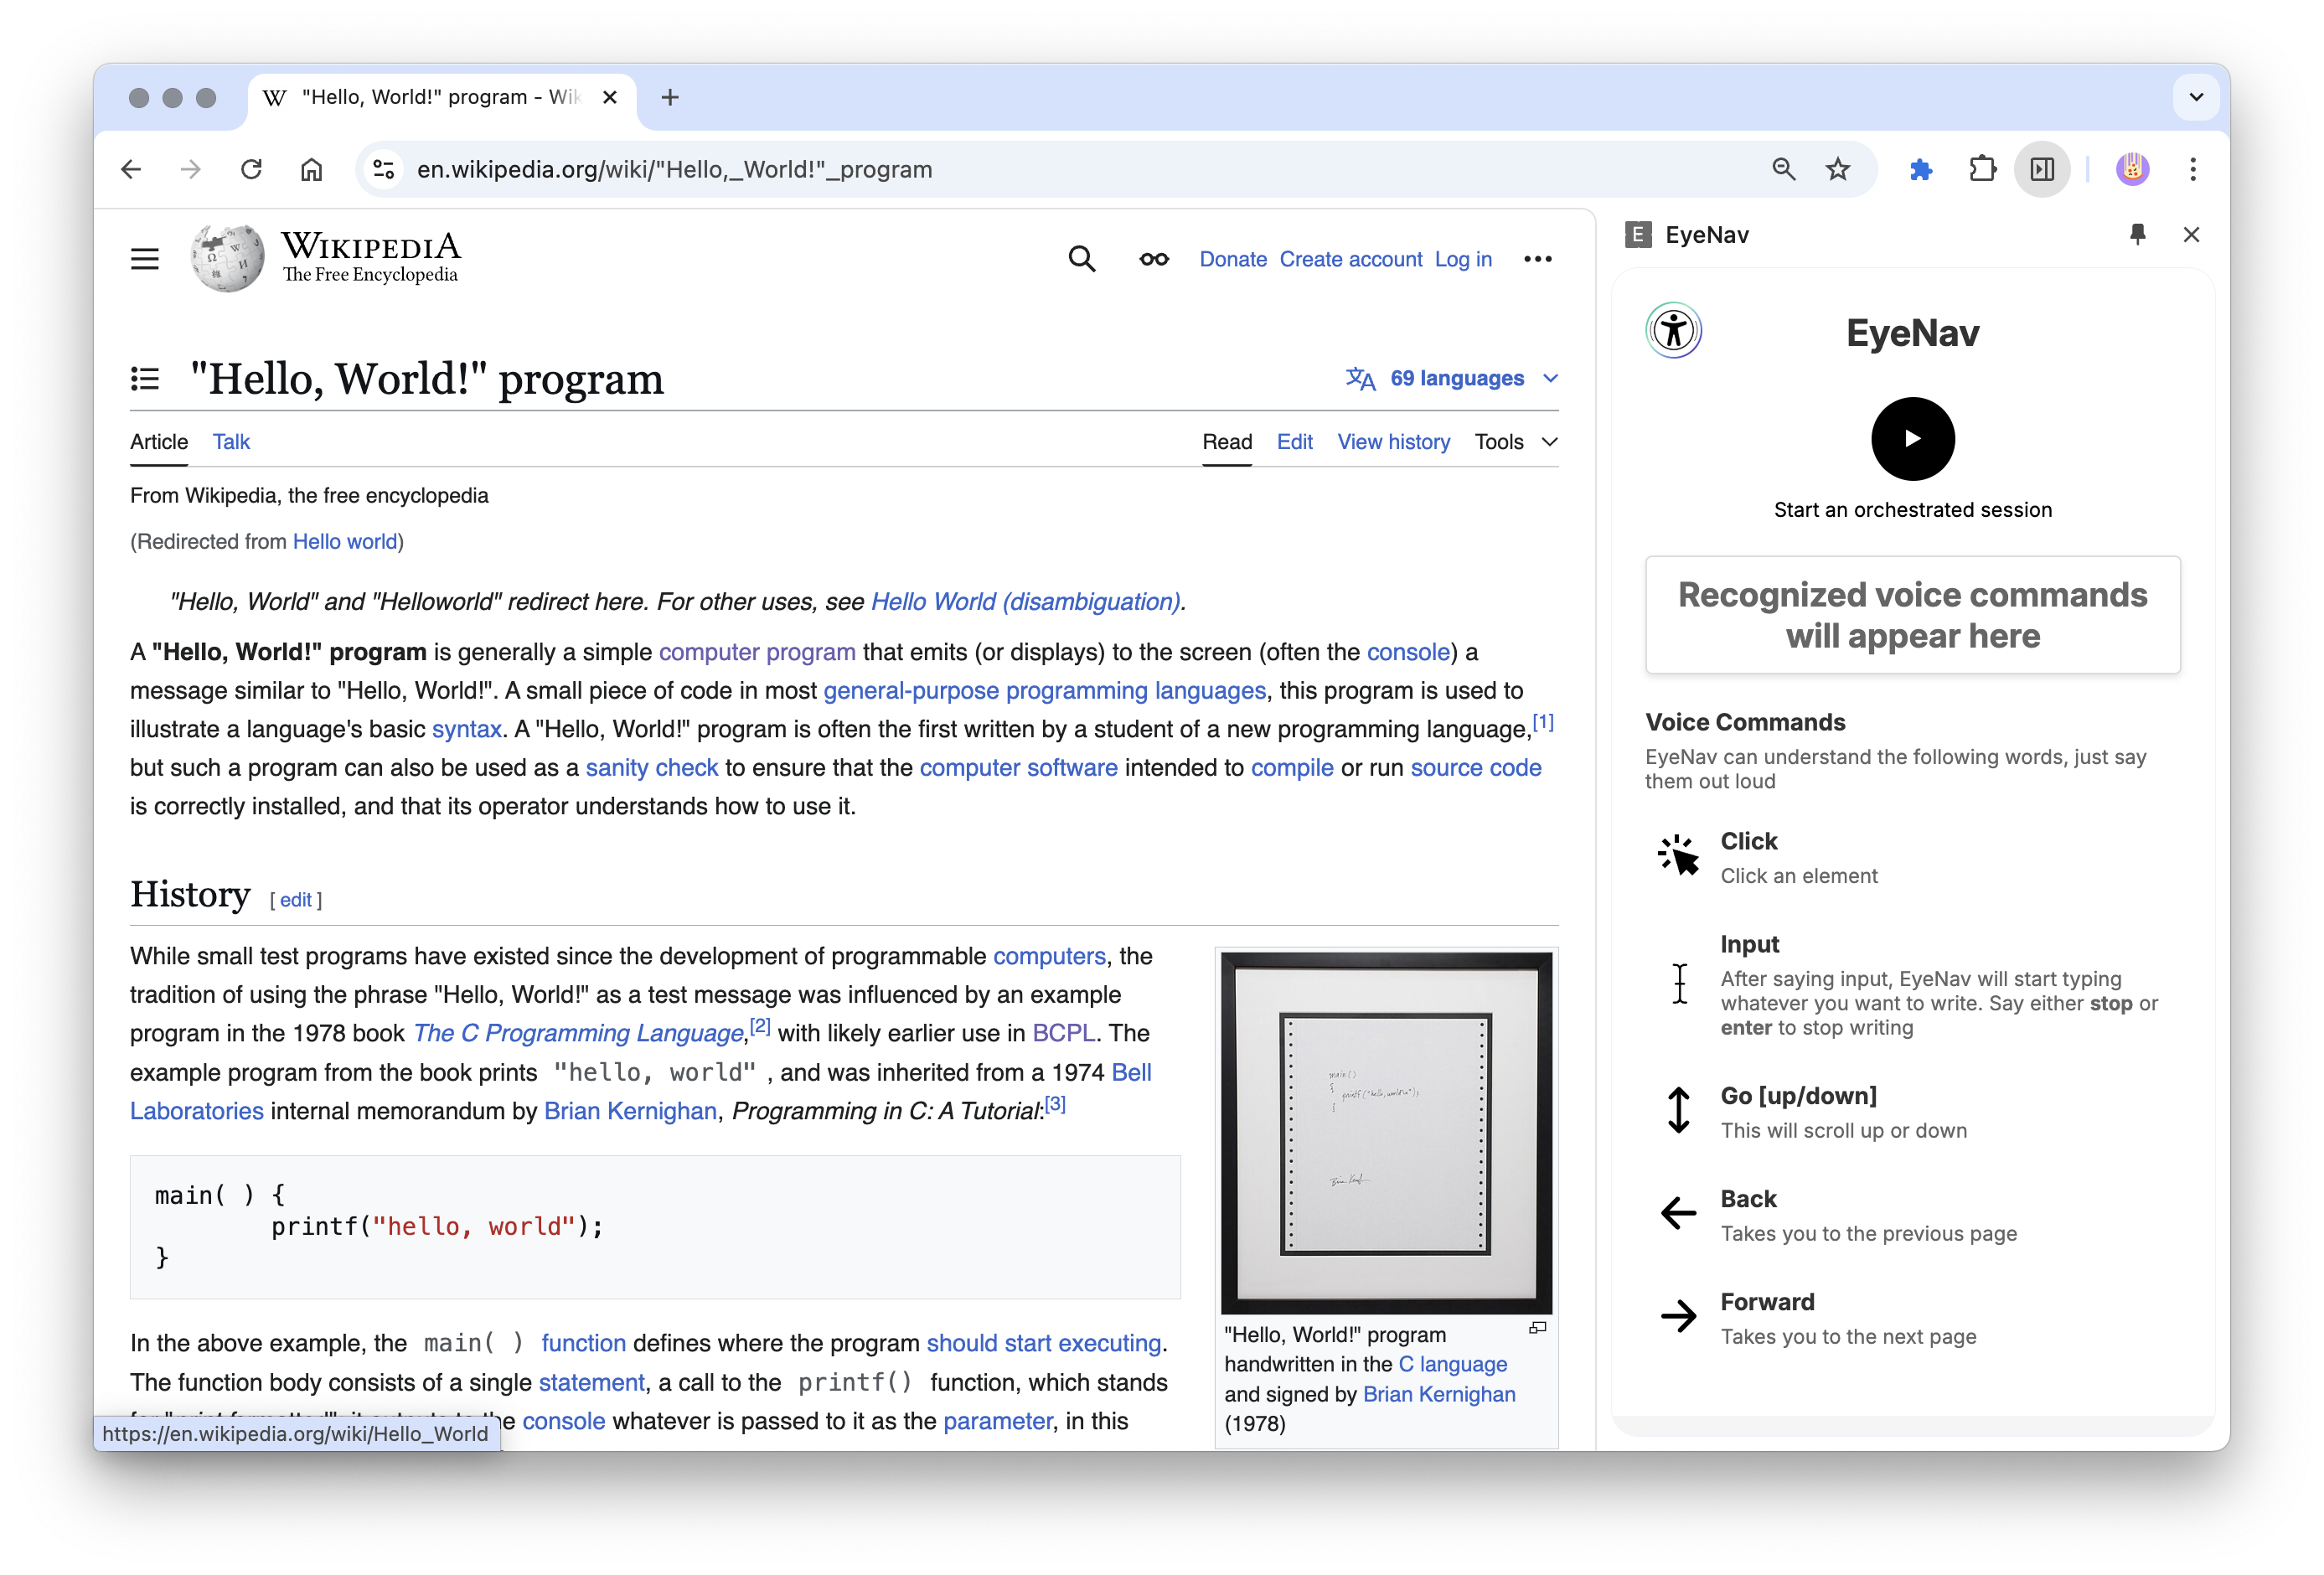
\includegraphics[width=1\textwidth]{images/screenshots/eyenav-1.png}
    \caption{Chrome extension}
    \label{fig:ss-1}
\end{figure}

\begin{figure*}[ht]
    \centering
    \begin{subfigure}[ht]{0.48\textwidth}
        \centering
        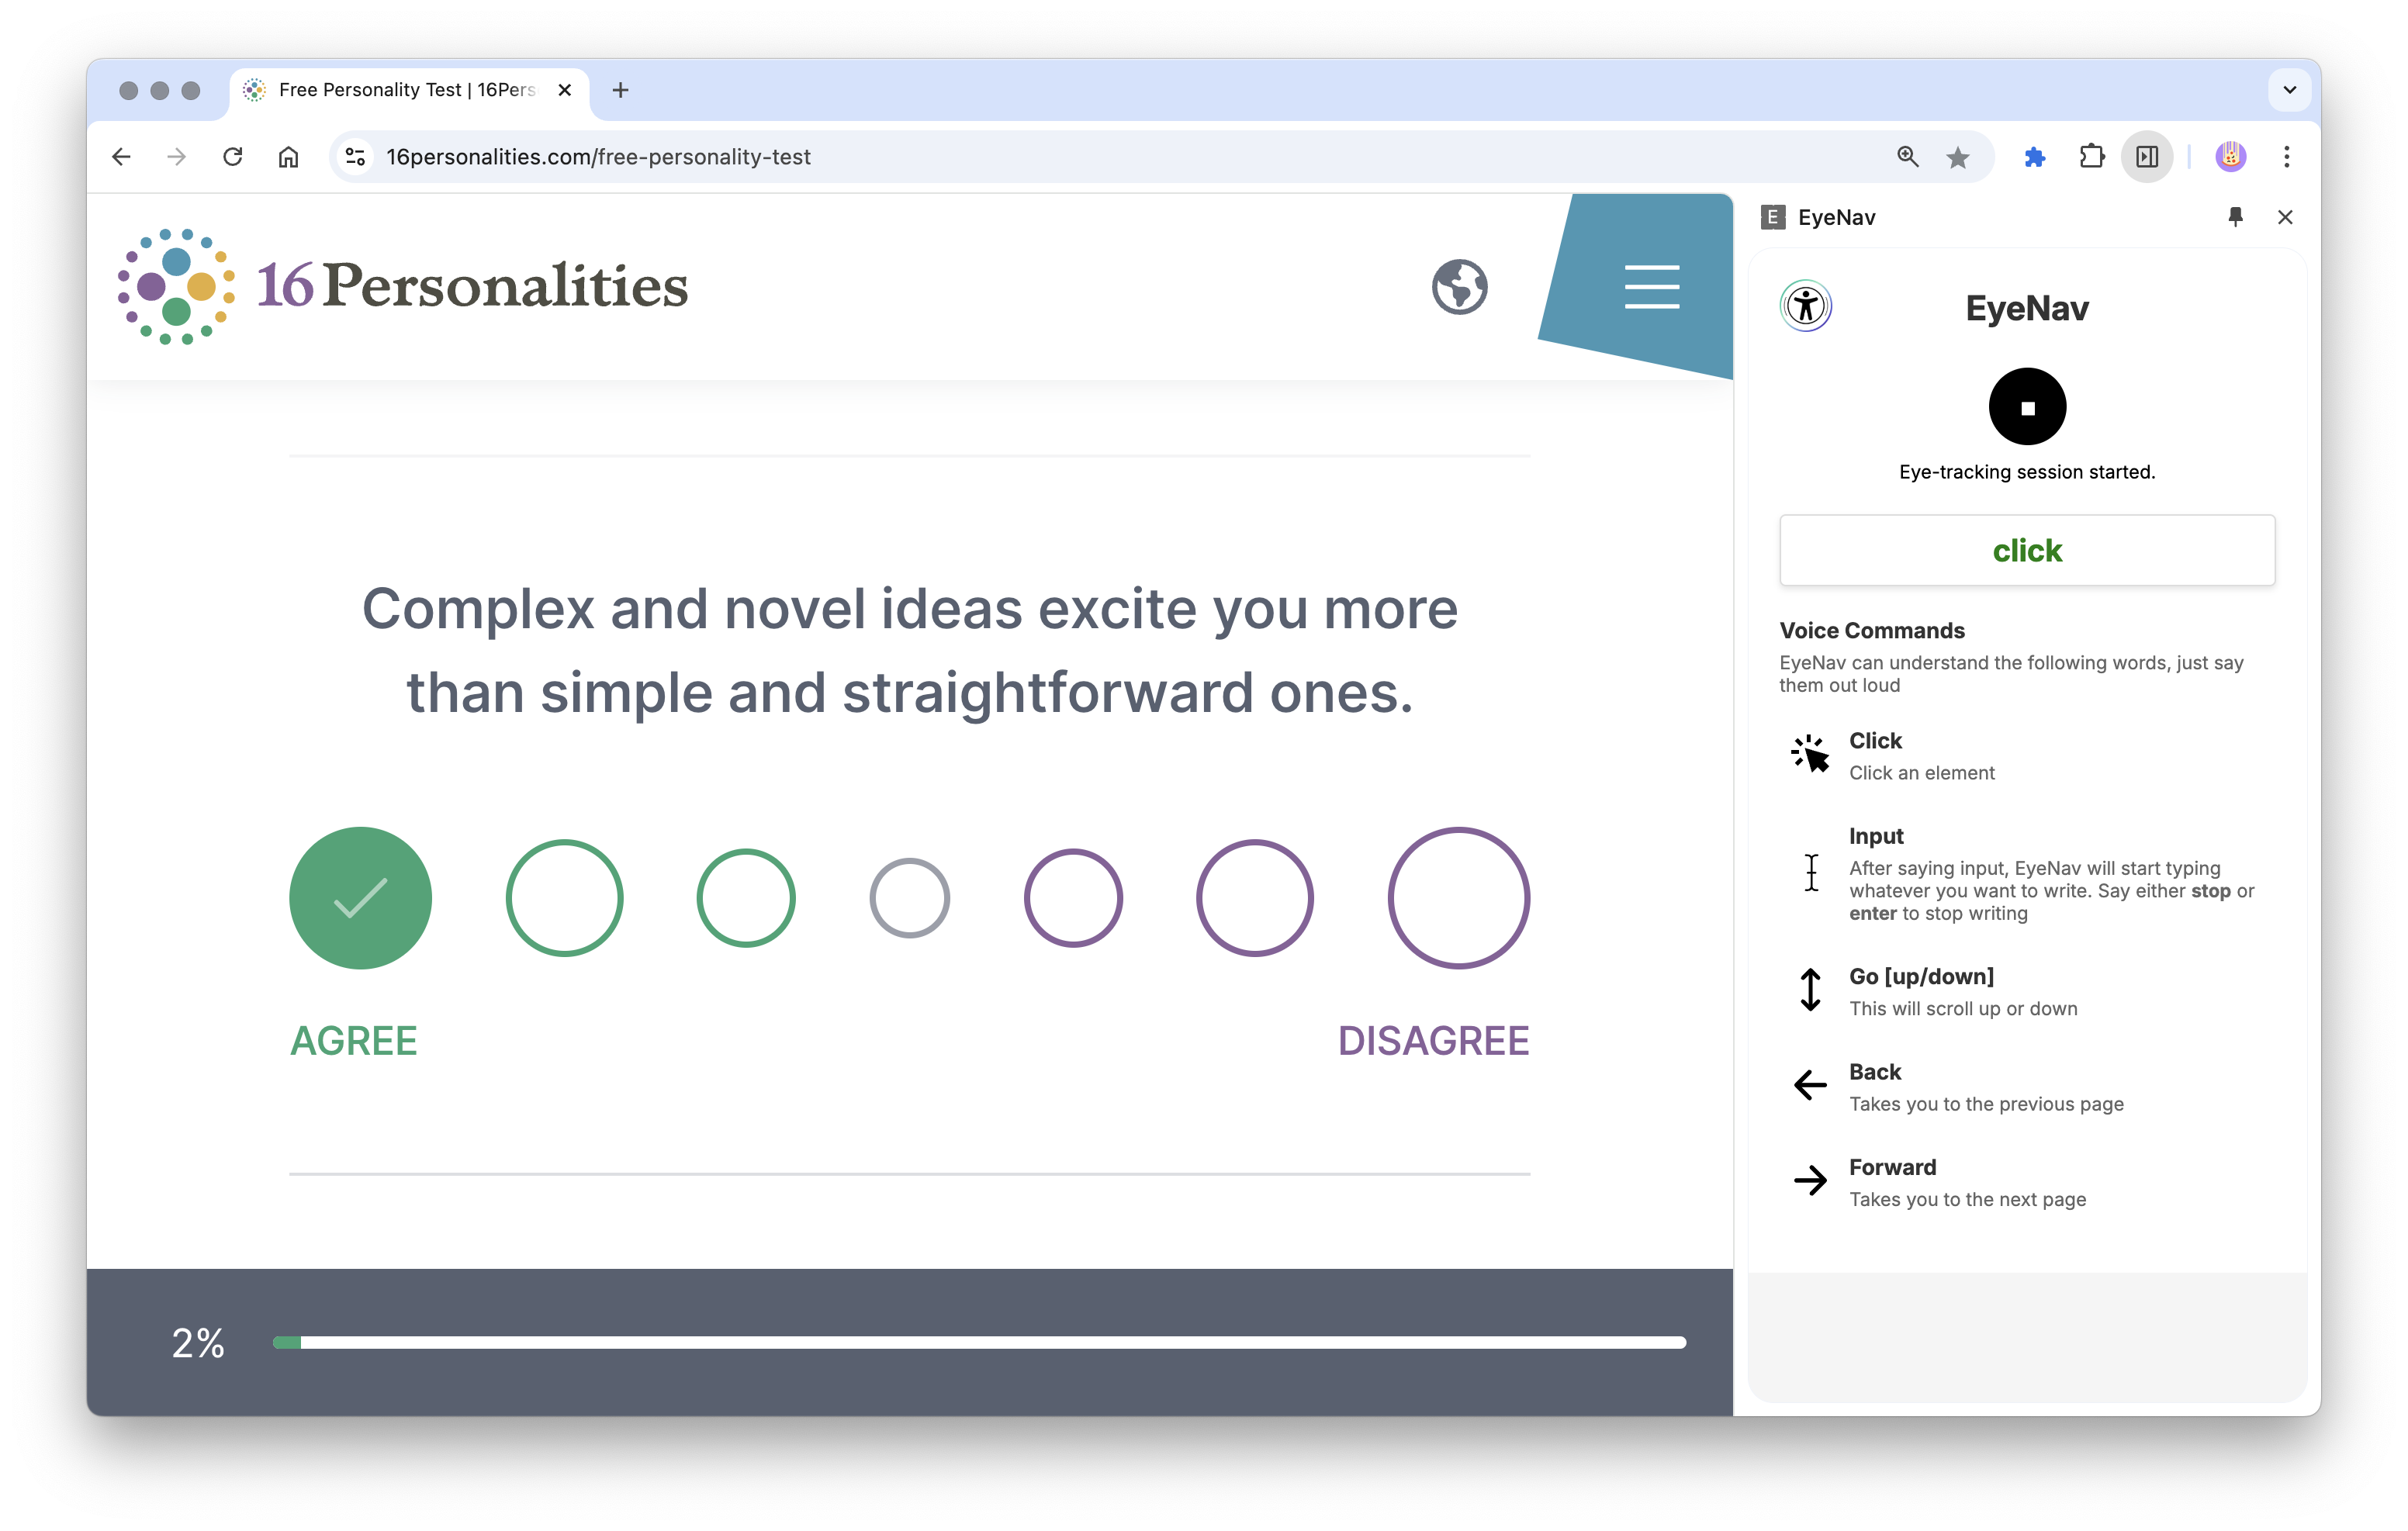
\includegraphics[width=\textwidth]{images/screenshots/eyenav-click.png}
        \caption{Clicking an item}
    \end{subfigure}
    ~ 
    \begin{subfigure}[ht]{0.48\textwidth}
        \centering
        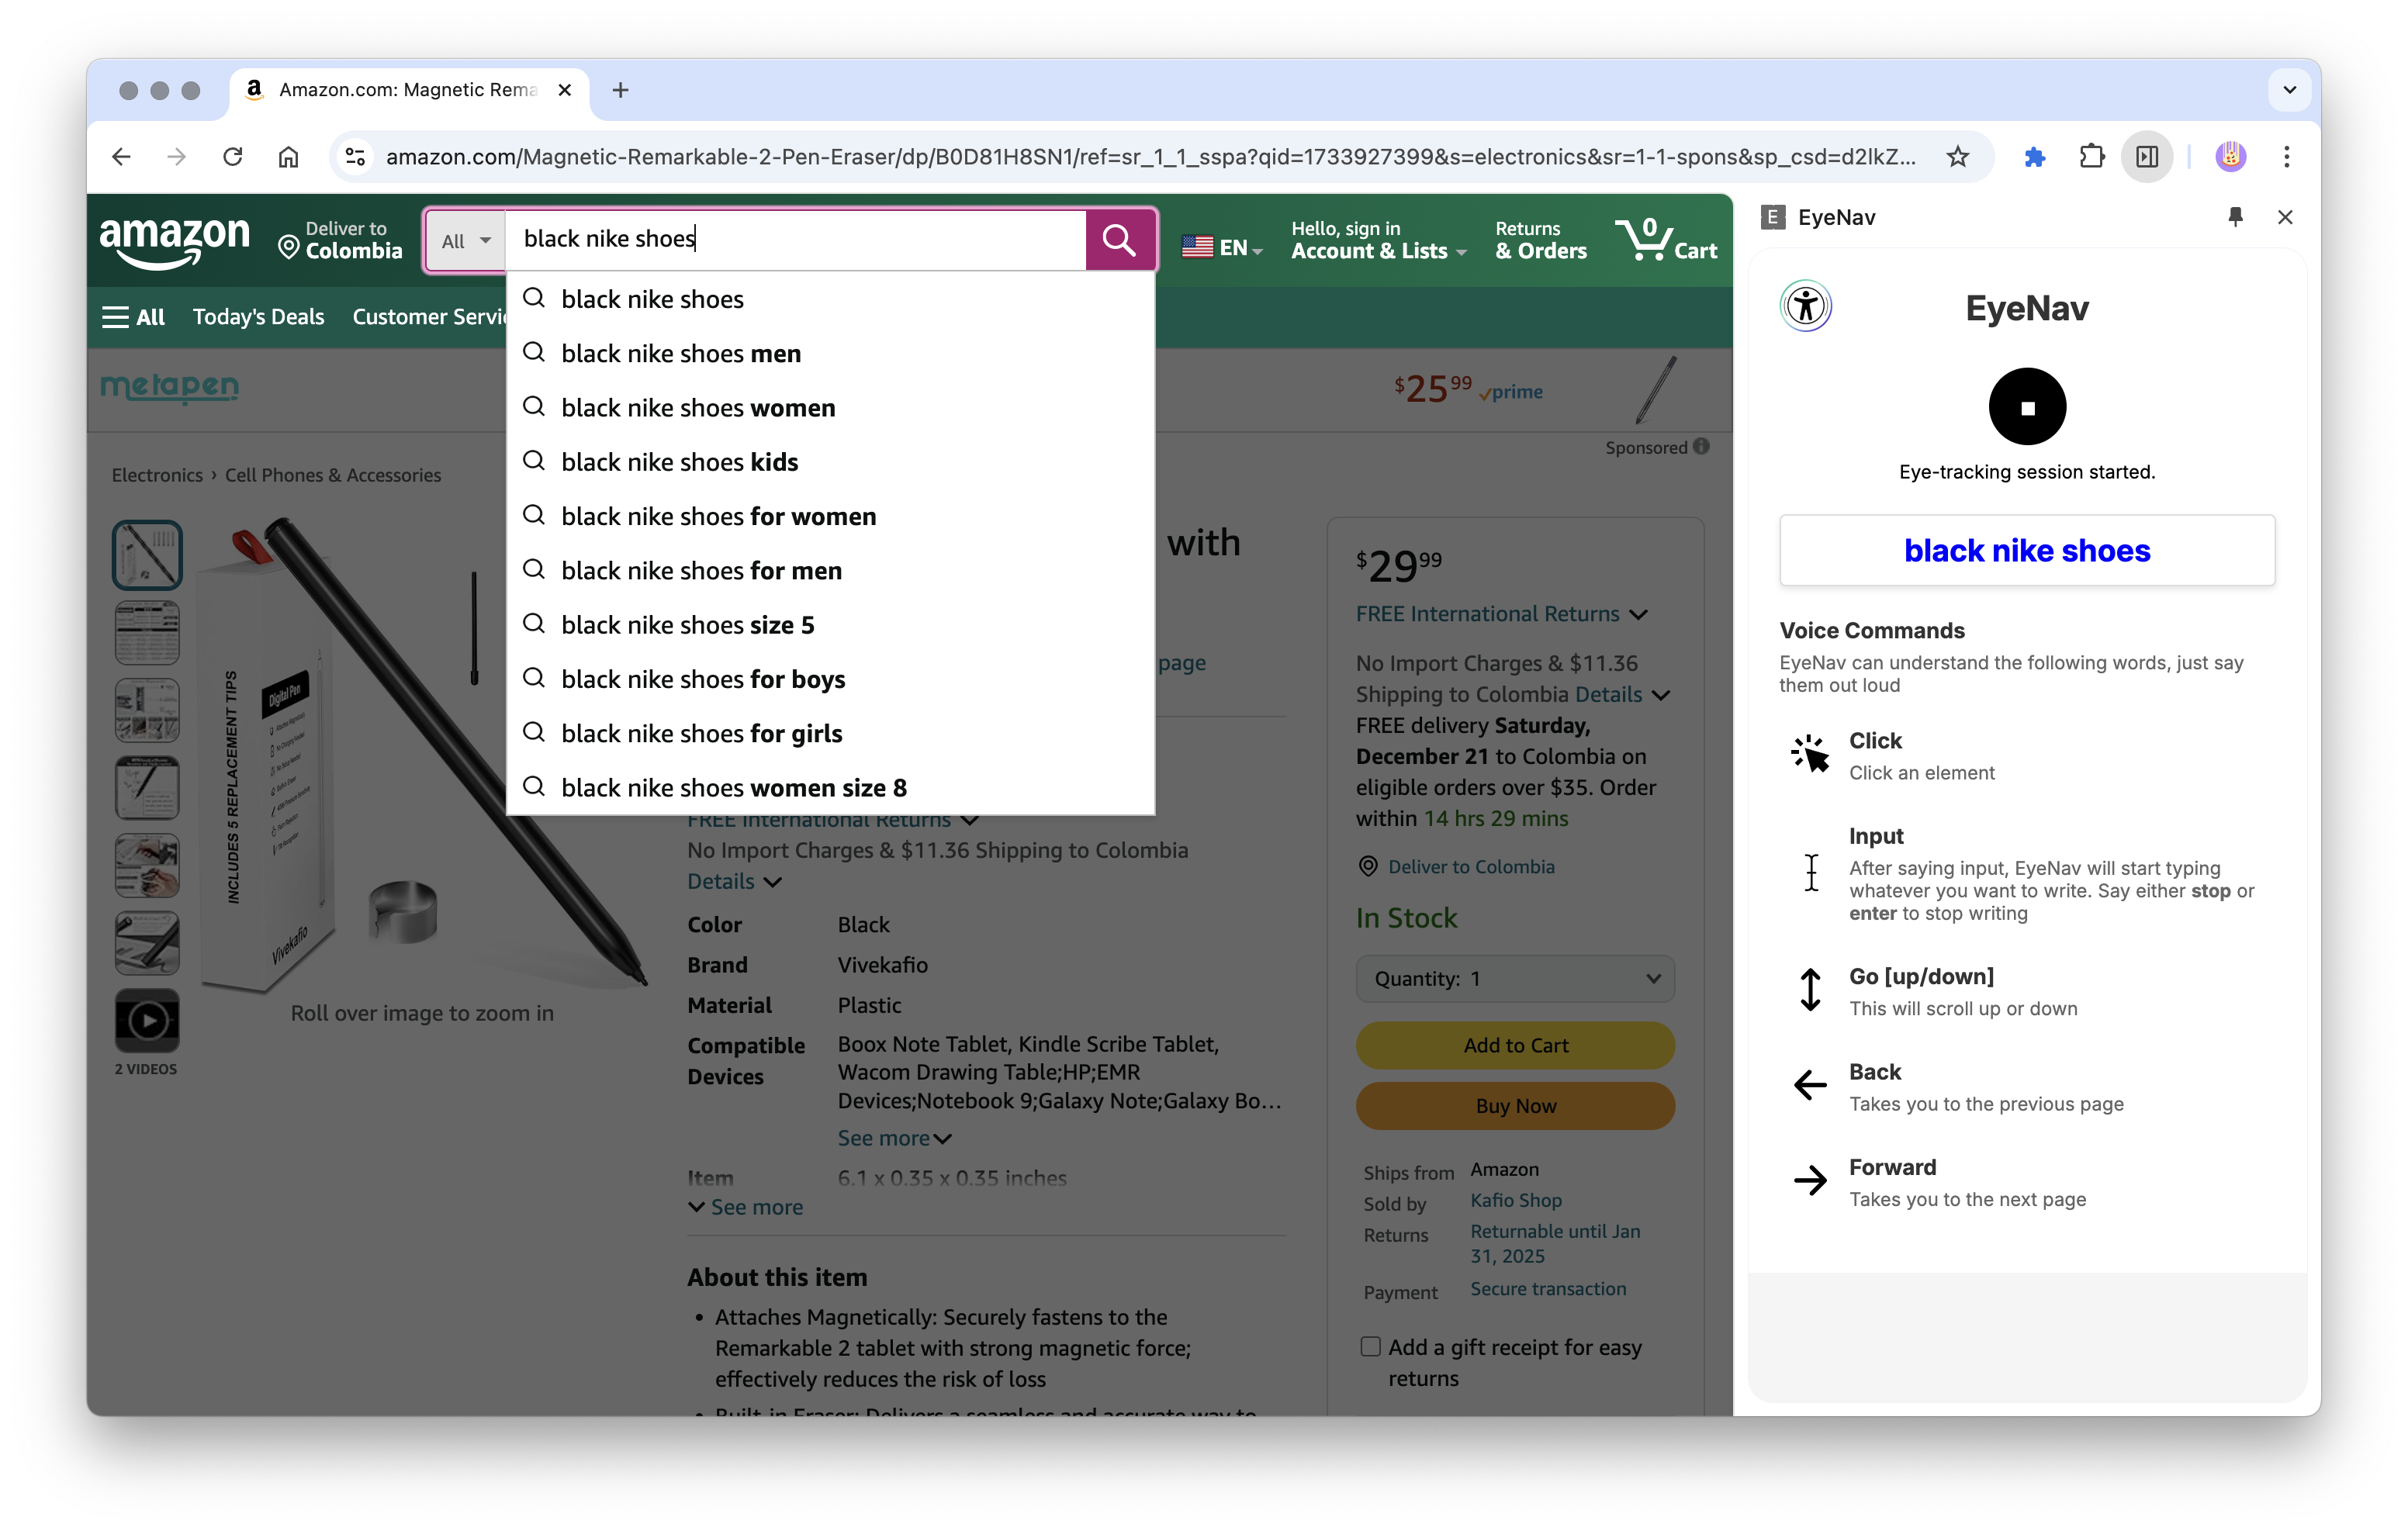
\includegraphics[width=\textwidth]{images/screenshots/eyenav-input.png}
        \caption{Inputting text}
    \end{subfigure}
    \caption{Other actions that can be done}
    \label{figs:ss-2-3}
\end{figure*}

Figures \ref{fig:ss-1} and \ref{figs:ss-2-3} illustrate the system in operation. The left side of the browser shows the webpage as it would appear in any web browser, while the right side features the side panel of the Chrome extension. This side panel must remain visible at all times for proper orchestration. Below the play button, the voice commands box displays recognized commands, with control words in green and input (typing mode) words in blue. At the bottom, a menu lists all available commands.

\subsection{Usability}

Usability in itself is not an absolute metric, and needs to be defined in particular contexts where it is being applied. In that sense, ways of measuring this non-functional requirement are not straight-forward and do not depend on a single method, but are rather cualitative data that need to be analysed in this way.

\subsubsection{System Usabillity Scale}

The system usability scale (SUS) is useful for understanding broad and general measurements of usability. Proposed by \cite{art:sus-1996}, this scale is widely used in systems engineering, and consists of 10 questions that the user will assess subjectively, but ultimately can point out how the system performed in three points:

\begin{itemize}
    \item effectiveness (the ability of users to complete tasks using the system, and the quality of the output of those tasks)
    \item efficiency (the level of resource consumed in performing tasks)
    \item satisfaction (users subjective reactions to using the system). \citep{art:sus-1996}
\end{itemize}

These are the statements proposed in the scale, where the subject can mark from 1 (strongly disagree) to 5 (strongly agree):

\begin{enumerate}[label=\textbf{\arabic*.}]
    \item I would like to use this system frequently. \hfill \underline{1 \quad 2 \quad 3 \quad 4 \quad 5}
    \item I found the system unnecessarily complex. \hfill \underline{1 \quad 2 \quad 3 \quad 4 \quad 5}
    \item I thought the system was easy to use. \hfill \underline{1 \quad 2 \quad 3 \quad 4 \quad 5}
    \item I think I would need technical support to use this system. \hfill \underline{1 \quad 2 \quad 3 \quad 4 \quad 5}
    \item The functions of the system were well integrated. \hfill \underline{1 \quad 2 \quad 3 \quad 4 \quad 5}
    \item There was too much inconsistency in the system. \hfill \underline{1 \quad 2 \quad 3 \quad 4 \quad 5}
    \item Most people would learn to use this system very quickly. \hfill \underline{1 \quad 2 \quad 3 \quad 4 \quad 5}
    \item I found the system very cumbersome to use. \hfill \underline{1 \quad 2 \quad 3 \quad 4 \quad 5}
    \item I felt very confident using the system. \hfill \underline{1 \quad 2 \quad 3 \quad 4 \quad 5}
    \item I needed to learn a lot of things before I could get going with this system. \hfill \underline{1 \quad 2 \quad 3 \quad 4 \quad 5}
\end{enumerate}

SUS have scores ranging from 0 to 100. Each individual score can be calculated like formula \ref{eq:sus} shows, where each $s_n$ represents each statement

\begin{equation}
    2.5 \left(20 \sum(s_1,s_3,s_5,s_7,s_9) - \sum(s_2,s_4,s_6,s_8,s_{10})\right) \label{eq:sus}
\end{equation}

Furthermore, in the usability tests conducted, the average SUS was \verb|76.7|, with the highest score being \verb|95| and the lowest being \verb|55|. Indicating that the system was found to be quite usable.


\subsubsection{User Feedback}
Another method to evaluate the system's usability was through user interviews. Key insights from these interviews include:

\begin{itemize}
    \item Scenario-specific usability: The navigability and ease of use of the system are directly related to the specific scenario or webpage being interacted with. Users found it easier to use when performing straightforward tasks like purchasing a product or reading news, but more challenging when completing complex actions such as filling out forms.
    \item Icon size: The ease of reaching icons using eye-tracking is highly dependent on their size. Larger icons are generally easier to navigate to.
    \item Environmental conditions: These significantly impact the system's usability, especially due to its reliance on voice recognition. In noisy environments, users found the system harder and less enjoyable to use.
    \item Interaction accuracy: Users expressed a desire for a feature that indicates the exact element the system is about to click, which could enhance interaction accuracy.
    \item User comfort: Most users felt comfortable using their voice and eyesight for interaction, describing this method as intuitive and user-friendly.
    \item Response time: The response time for each action was deemed satisfactory by all users, indicating no significant delays.
    \item Voice control: Voice control seemed to be easier whenever control words were clearer and shorter. For instance, when the first prototype was developed, the user had to say in units how much they wanted to scroll, like "scroll down five units". This became a hassle and was ultimately decided that scrolling would be done in an arbitrary number of units that is intuitive.
\end{itemize}


\subsection{Accessibility}

\subsubsection{User Feedback}

\begin{itemize}
    \item According to \cite{techreport:webaim-2024}, \verb|95.9%| of webpages have at least one detectable accessibility error. Accessibility is an attribute of the webpage itself, so many tester users felt that this system indeed leverages a new way of interacting with webpages. However, to become more accessible, it would need to align with the actual design of the webpage, such as making icons easier to reach and text more readable.
    \item Due to the scope and time limitations of the project, testing with individuals with motor impairments was not possible. However, all users who tested the system suggested that this method of interaction could be beneficial for individuals with motor impairments. They even mentioned that if the system were more polished, they would consider using it regularly to be more productive.
\end{itemize}


\subsection{Test Script Generation}

The system's tests are a series of actions recorded during user interactions. These actions are documented in Gherkin syntax, which are then interpreted and mapped to corresponding Webdriver actions that the testing module can replay. Below is an example of a test script:

\begin{lstlisting}
    Feature: Replay of session on Nov 11 at 02:48:38 PM

    @user1 @web
    Scenario: User interacts with the web page named "Amazon.com. Spend less. Smile more."
    
        Given I navigate to page "https://www.amazon.com/"
        And I click on tag with id "twotabsearchtextbox"
        And I input "nike black shoes"
        And I click on tag with id "nav-search-submit-button"
        And I scroll down
        And I click on tag with xpath "/html[1]/body[1]/div[1]/div[1]/div[1]/div[1]/div[1]/span[1]/div[1]/div[9]/div[1]/div[1]/span[1]/div[1]/div[1]/div[1]/span[1]/a[1]/div[1]"
\end{lstlisting}

These actions are replayable thanks to the Kraken module. However, as webpages dynamically change and evolve, these tests have a limited lifespan. Despite this, they can be valuable for specific testing scenarios. For example, they can help determine how a webpage behaves when its size changes, how many clicks are required to perform the same action, and whether the flow of actions breaks if the webpage layout changes.
